\chapter{Einleitung}
\section{NP-Vollst�ndigkeit}
Eine Sprache B ist \textbf{NP-Vollst\"andig} wenn gilt:
\begin{enumerate}
	\item $B \in NP$
	\item $\forall A \in NP: A \prec_p B$
\end{enumerate}

Notiz:\\
$A \prec_p B$ : $A$ ist polynomialzeitreduzierbar auf $B$

\section{Polynomialzeitreduktion}
Eine Sprache $A$ ist polynomialzeitreduzierbar auf Sprache $B$, $A \prec_p B$, wenn eine in polynomialer Zeit berechenbare Funktion $f:\Sigma^* \to \Sigma^*$ existiert, f�r die gilt:\\
$\forall w:$
	$w \in A \iff f(w) \in B$

Die Funktion $f$ hei�t dann Polynomialzeitreduktion von $A$ nach $B$.

\section{Definition 3SAT}
Spezialform des Erf\"ullbarkeitsproblems
\begin{itemize}
	\item Literal:\\
	$x_i$ oder $\overline{x_i}$
	\item Variable:\\
	$x_i$ (l: Anzahl der Variablen)
	\item Klausel:\\
	$(x_1 \lor \overline{x_2} \lor \overline{x_3} \lor x_4)$ (k: Anzahl der Klauseln)
	\item CNF-Formel(cnf-formula - conjunctive normal form):\\
	$(x_1 \lor \overline{x_2} \lor \overline{x_3} \lor x_4) \land (x_3 \lor \overline{x_5} \lor x_6) \land (x_3 \lor \overline{x_6})$
	\item $\phi$: $(x_1 \lor \overline{x_2} \lor \overline{x_3}) \land (\overline{x_2} \lor x_4 \lor ...) \land ... \land (\overline{x_3} \lor ... \lor ...)$
\end{itemize}

$3SAT = \left\{ \right. \langle \phi \rangle | \phi$ ist eine erf�llbare 3CNF-Formel$\left. \right\}$

$\phi = 1 \iff \forall c_j$: mindestens ein Literal ist $true$ 

\chapter{Hamilton-Pfad-Problem}
\section{Definition}
\begin{itemize}
	\item Geht durch jeden Knoten genau einmal
	\item Startet in s
	\item Endet in t
\end{itemize}

Notiz: Gesucht: Pfad von $s$ nach $t$, der durch jeden knoten genau einmal geht.

\section{Beweis Gerichtet}
\subsection{HAMPATH $\in$ NP}
Notiz: Eine nichtdeterministische Turingmaschine r�t das Ergebnis und Verwirft dann bzw. nimmt an.

\subsection{Konstruktion von G}
$\phi \to G$

\subsubsection{Darstellung Variable $x_i$}
\begin{center}
	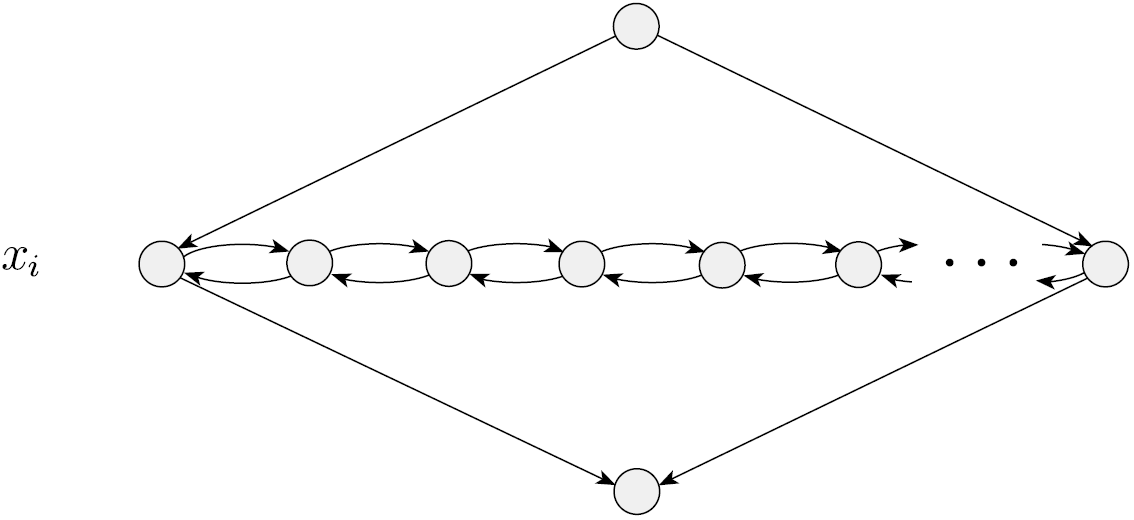
\includegraphics[width=14cm]{images/hampath/1}
\end{center}

\subsubsection{Darstellung Klausel $c_j$}
\begin{center}
	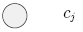
\includegraphics{images/hampath/2}
\end{center}

\subsubsection{High-level structure of G}
\begin{center}
	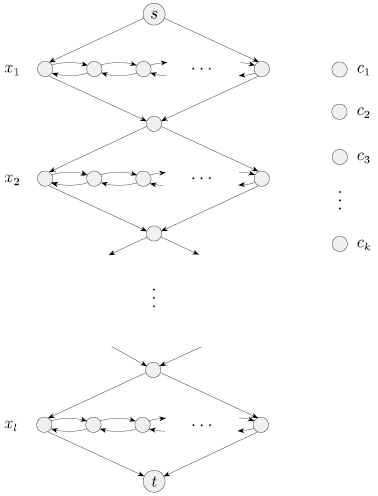
\includegraphics[width=14cm]{images/hampath/3}
\end{center}

\subsubsection{Horizontale Struktur im Diamant}
\begin{center}
	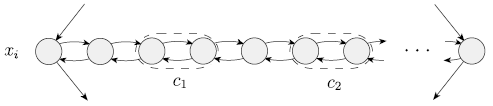
\includegraphics[width=14cm]{images/hampath/4}
\end{center}
$\left<3k+1\right>$ Knoten

\subsubsection{Zus\"atzliche Kanten wenn $x_i$ in $c_j$ ist}
\begin{center}
	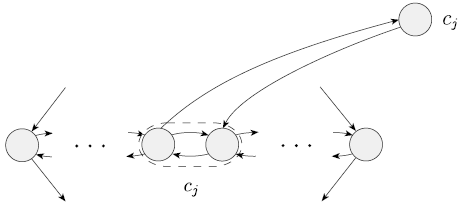
\includegraphics[width=14cm]{images/hampath/5}
\end{center}

Notiz: Am Beispiel von $\phi$ zeigen!

\subsubsection{Zus\"atzliche Kanten wenn $\overline{x_i}$ in $c_j$ ist}
\begin{center}
	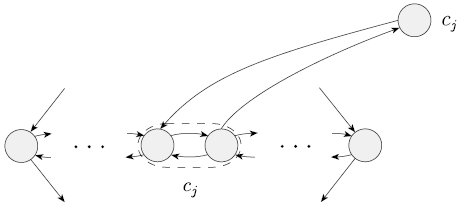
\includegraphics[width=14cm]{images/hampath/6}
\end{center}

\subsection{$\phi$ ist erf\"ullbar}

Notiz: Zun\"achst werden die Knoten $c_j$ ignoriert.

Notiz: Der Pfad geht von $s$ nach $t$ durch jeden Diamanten nach einander.

Notiz: Um alle Knoten zu treffen muss der Pfad entweder zig-zaggen oder zag-ziggen.

\subsubsection{Zig-zagging and Zag-zigging}
\begin{center}
	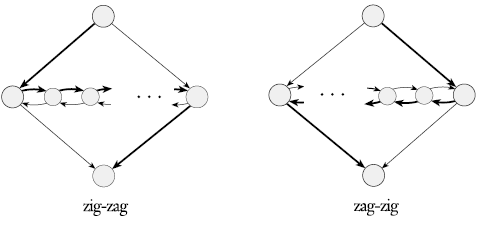
\includegraphics[width=14cm]{images/hampath/7}
\end{center}

Notiz: Zig-zagging wenn Variable $x_i=true$, Zag-zigging wenn Variable $x_i=false$

Notiz: Jetzt fehlen nurnoch die Knoten $c_j$.

Notiz: In jeder Klausel $c_j$ w\"ahlen wir einen Literal aus, dem wir $true$ zuweisen.

Notiz: Jeder wahre Literal in einer Klausel ist nur eine Option f�r einen Umweg \"uber einen Klauselnoten. $\to$ Es wird immer nur ein Umweg zu jedem Klauselknoten genommen. $\to$ Konstruktion von $G$ ist beendet.

\subsection{G hat einen HAMPATH}

\begin{itemize}
	\item HAMPATH muss normal sein, geht durch Diamanten von oben nach unten(ausgenommen von den Umwegen \"uber die Klauselknoten
	\item zig-zag $\to$ $x_i = true$, zag-zig $\to$ $x_i = false$
	\item Anhand dessen, wie der Umweg \"uber einen Klauselknoten genommen wird kann man erkennen welcher Literal der Klausel wahr ist
	\item Hampath ist normal zeigen
\end{itemize}

\begin{center}
	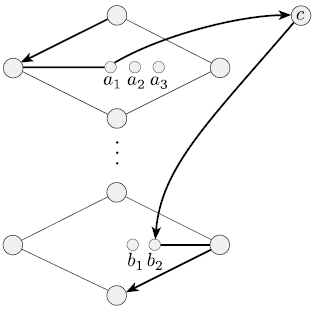
\includegraphics[width=14cm]{images/hampath/8}
\end{center}

\subsubsection{Laufzeit}
Notiz: Anhand des Graphen erl\"autern(Anzahl Knoten)

\subsection{Ungerichtet}
\TODO{muss der auch rein?}

\chapter{SUBSET-SUM-Problem}
\section{Definition}
\begin{itemize}
	\item Integer-Arithmetik (dezimal)
	\item Menge von Zahlen $S$: $x_1,...,x_k$
	\item Target $t$
	\item Kann $t$ durch ein Subset von $S$ erreicht werden?
\end{itemize}

\section{Beweis}
3SAT $\prec_p$ SUBSET-SUM

$\phi$: $(x_1 \lor \overline{x_2} \lor \overline{x_3}) \land (\overline{x_2} \lor x_4 \lor ...) \land ... \land (\overline{x_3} \lor ... \lor ...)$

\subsection{SUBSET-SUM $\in$ NP}
Notiz: Eine nichtdeterministische Turingmaschine r�t das Ergebnis und Verwirft dann bzw. nimmt an.

\subsection{Konstruktion der Tabelle}
\begin{itemize}
	\item Elemente aus $S$ und die Zahl $t$ sind die Zeilen der Tabelle (in Dezimaldarstellung)
	\item Die Zeilen oberhalb des Doppellinie sind $y_1, z_1, y_2, z_2,...,y_l, z_l$ und $g_1, h_1, g_2, h_2,..., g_k, h_k$
	\item Unter der Doppellinie ist $t$, $l$ 1 gefolgt von $k$ 3
	\item $S$ hat ein Paar $y_i, z_i$ f\"ur jede Variable $x_i$ in $\phi$
	\item linke Seite: 1 gefolgt von $l-i$ 0
	\item rechte Seite: $1 \iff c_j$ $x_i$ beinhaltet, $0 \iff c_j$ $\overline{x_i}$ beinhaltet
	\item nicht gef�llte Stellen sind $0$
	\item $g_j, h_j$ f\"ur jede Klausel $c_j$
	\item $g_j = h_j$, 1 gefolgt von $k-j$ 0
	\item Kein Carry m\"oglich
\end{itemize}

\begin{tabular}{c | c c c c c c | c c c c}
 & 1 & 2 & 3 & 4 & ... & l & $c_1$ & $c_2$ & ... & $c_k$ \\
\hline
$y_1$ & 1 & 0 & 0 & 0 & ... & 0 & 1 & 0 & ... & 0 \\ 
$z_1$ & 1 & 0 & 0 & 0 & ... & 0 & 0 & 0 & ... & 0 \\
$y_2$ &   & 1 & 0 & 0 & ... & 0 & 0 & 0 & ... & 0 \\
$z_2$ &   & 1 & 0 & 0 & ... & 0 & 1 & 1 & ... & 0 \\
$y_3$ &   &   & 1 & 0 & ... & 0 & 0 & 0 & ... & 0 \\
$z_3$ &   &   & 1 & 0 & ... & 0 & 1 & 0 & ... & 1 \\
... &   &   &   &   & ... &   &   &   & ... &   \\
$y_l$ &   &   &   &   &  & 1 & 0 & 0 & ... & 0 \\
$z_l$ &   &   &   &   &  & 1 & 0 & 0 & ... & 0 \\
\hline
$g_1$ &   &   &   &   &  & 1 & 0 & 0 & ... & 0 \\
$h_1$ &   &   &   &   &  & 1 & 0 & 0 & ... & 0 \\
$g_2$ &   &   &   &   &  &   & 1 & 0 & ... & 0 \\
$h_2$ &   &   &   &   &  &   & 1 & 0 & ... & 0 \\
... &   &   &   &   & ... &   &   &   & ... &   \\
$g_k$ &   &   &   &   &  &   &   &   &  & 1 \\
$h_k$ &   &   &   &   &  &   &   &   &  & 1 \\
\hline
\hline
t & 1 & 1 & 1 & 1 &... & 1 & 3 & 3 & ... & 3\\
\end{tabular}

\subsection{Annahme}
Es existiert eine Konfiguration f�r die $\phi$ erf\"ullt ist.

\begin{itemize}
	\item W\"ahle $y_i$ wenn Variable $x_i$ wahr ist, ansonsten $z_i$
	\item Summe ergibt nur 1 auf der linken Seite, auf der rechten Seite nur 1 bis 3
	\item $g$ und $h$ w\"ahlen bis $t$ erreicht
\end{itemize}

\subsection{Annahme}
Ein Subset von $S$ ergibt $t$.

\begin{itemize}
	\item $y_i$ oder $z_i$ um 1 f\"ur linke Seite zu bekommen
	\item Wenn $y_i$ im Subset dann $x_i = true$, ansonsten $false$
	\item Summe der rechten Seite ist immer 3, maximal 2 k\"onnen von $g$ und $h$ kommen, daher alle $c_j$ wahr
	\item Wenn $y_i$ dann ist $x_i$ in $c_j$ und wird $true$ gesetzt, wenn $z_i$ dann $\overline{x_i}$ in $c_j$ und $x_i$ wird aus $false$ gesetzt
	\item Daher ist $\phi$ wahr
\end{itemize}

\subsection{Laufzeit}
Tabelle hat etwa eine Gr\"o�e von $(l + k)^2$\\
Jeder Eintrag ist leicht zu berechnen $\Rightarrow O(n^2)$